% Chapter 4

\chapter{CA Guide Frontend} % Main chapter title

\label{frontend} % For referencing the chapter elsewhere, use \ref{Chapter1} 

\lhead{Chapter 4. \emph{Museum Guide Frontend}} % This is for the header on each page - perhaps a shortened title

%----------------------------------------------------------------------------------------

\section{Architecture}

A fundamental requirement for the CA Guide frontend, the mobile application, is the ability to automatically test the single layers using recorded sensor data and comparing it with it's expected result.

To achieve this level of testability, virtual sensors are introduced at three different levels of abstraction:
 
\begin{figure}[H]
\centering
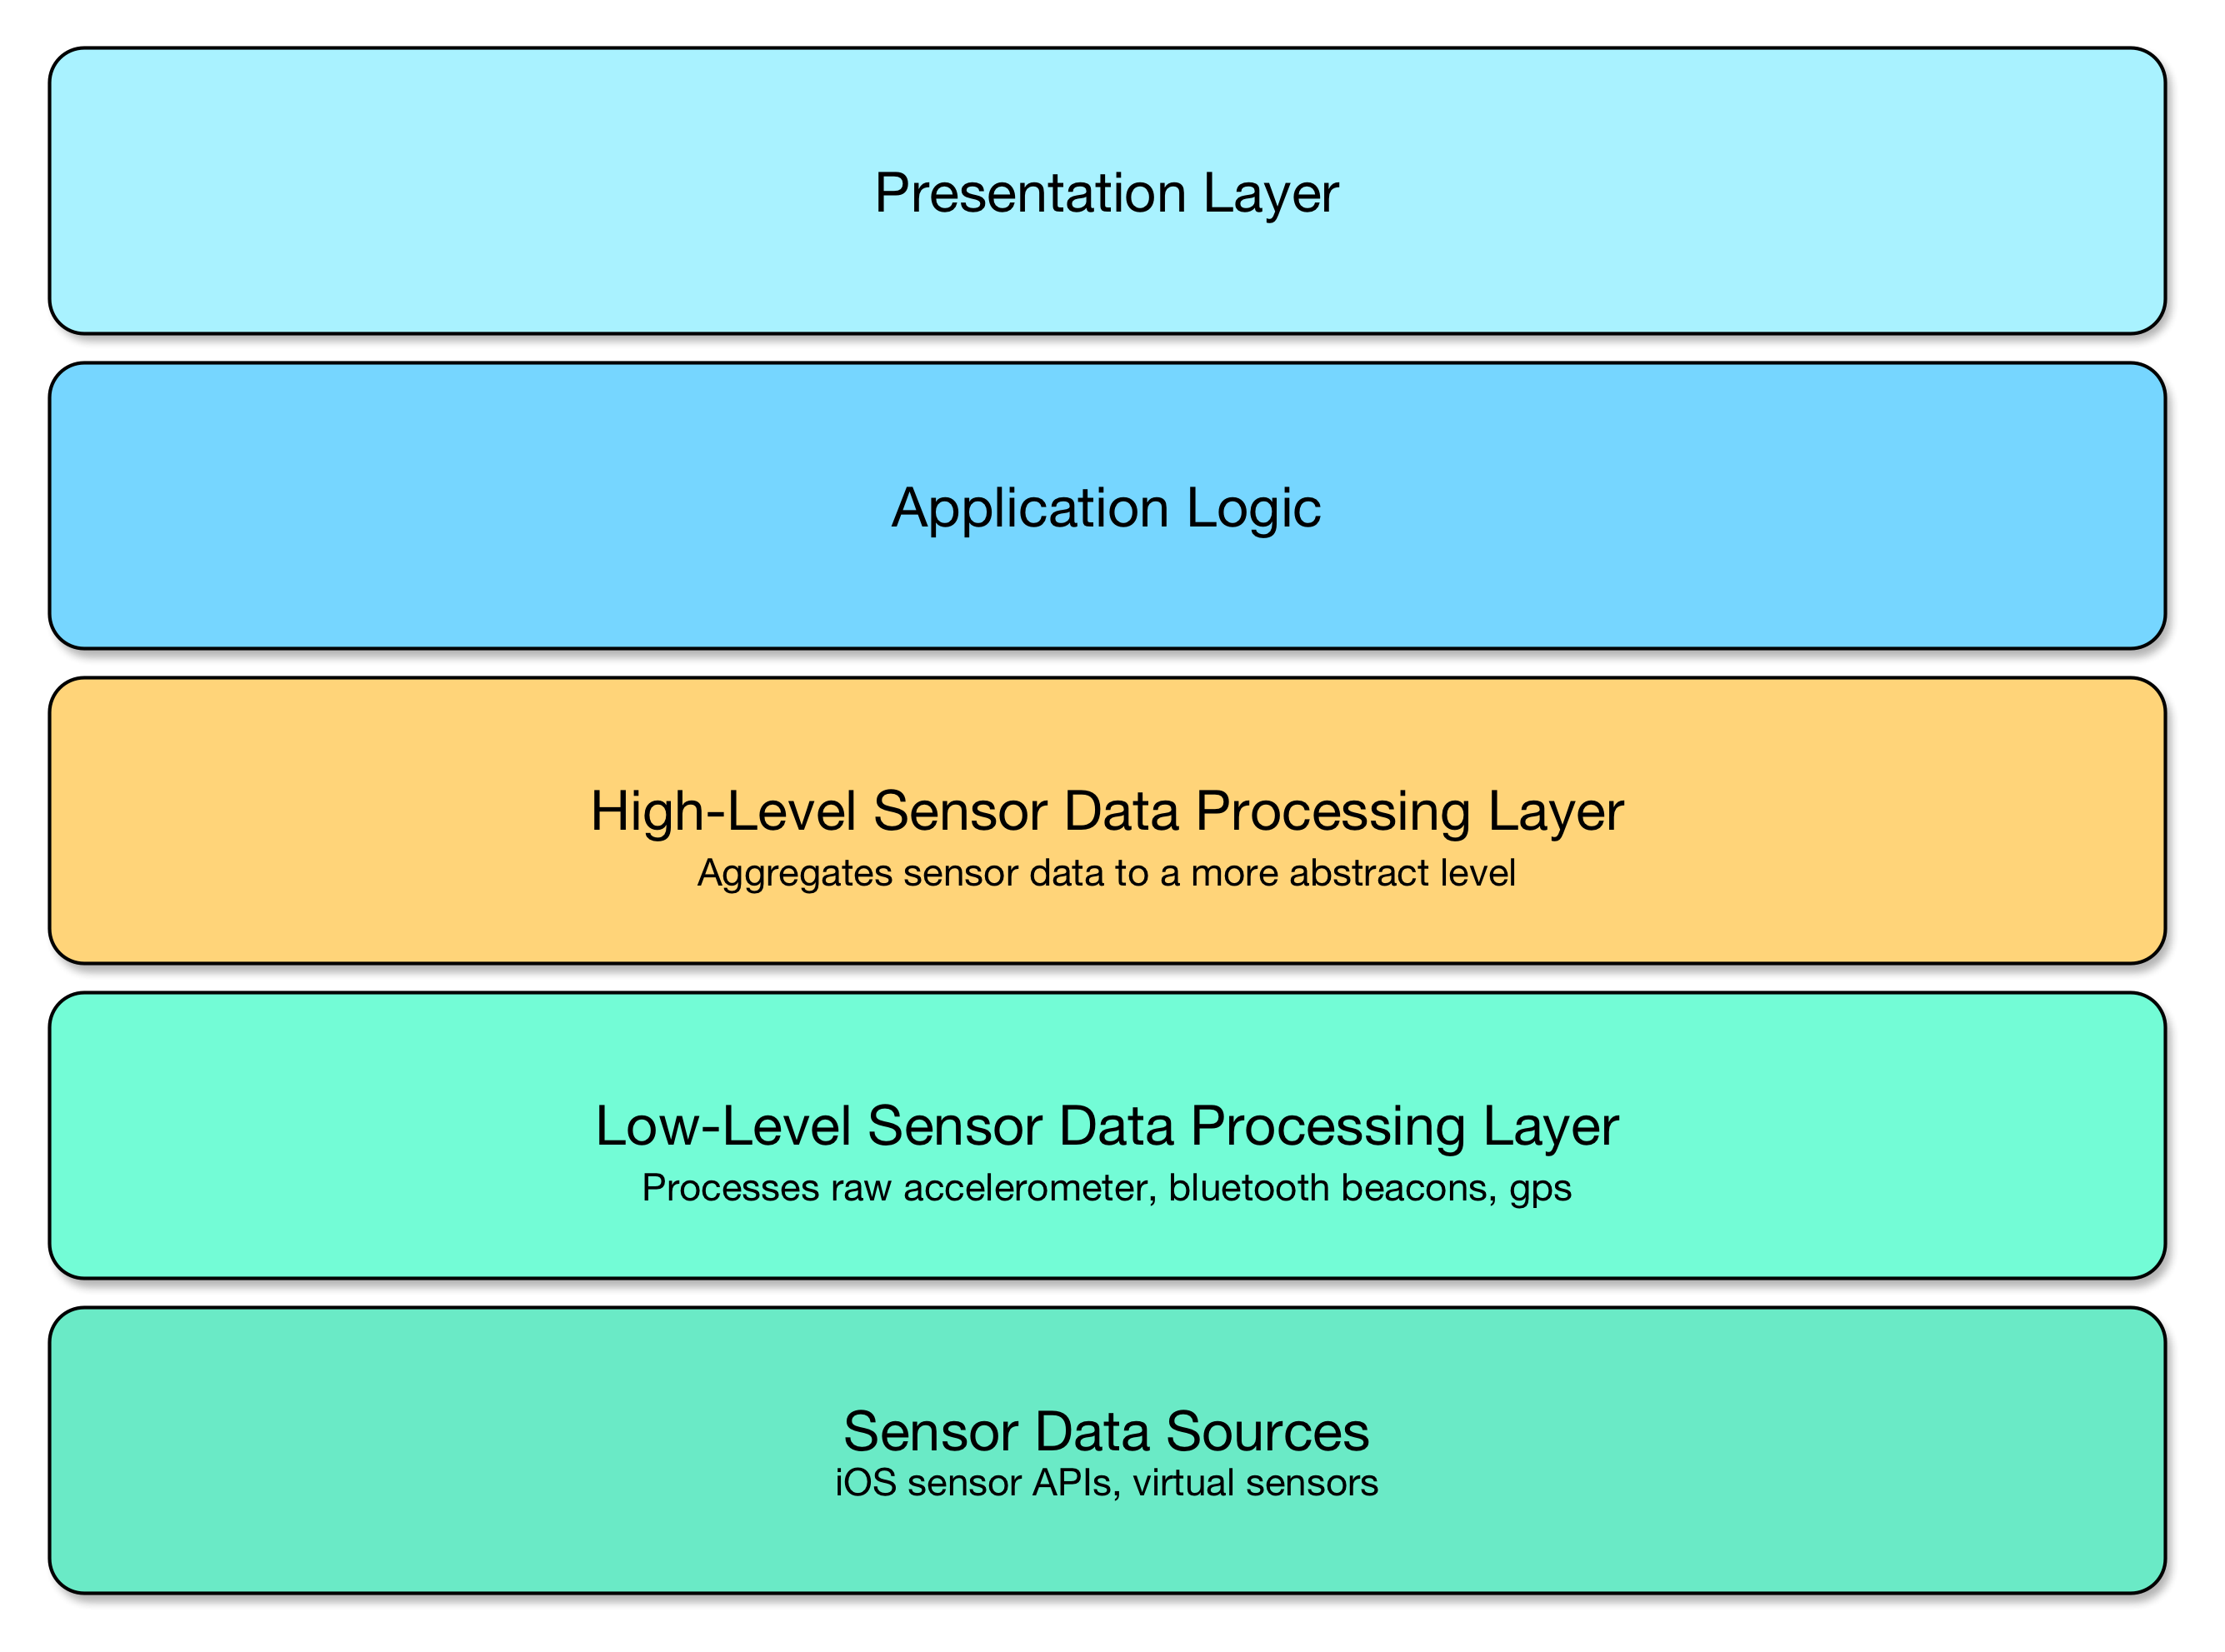
\includegraphics[width=0.9\textwidth]{layers-guide-app.png}
\caption{Layer Model of the Museum Guide Application}
\end{figure}

\begin{figure}[H]
\centering
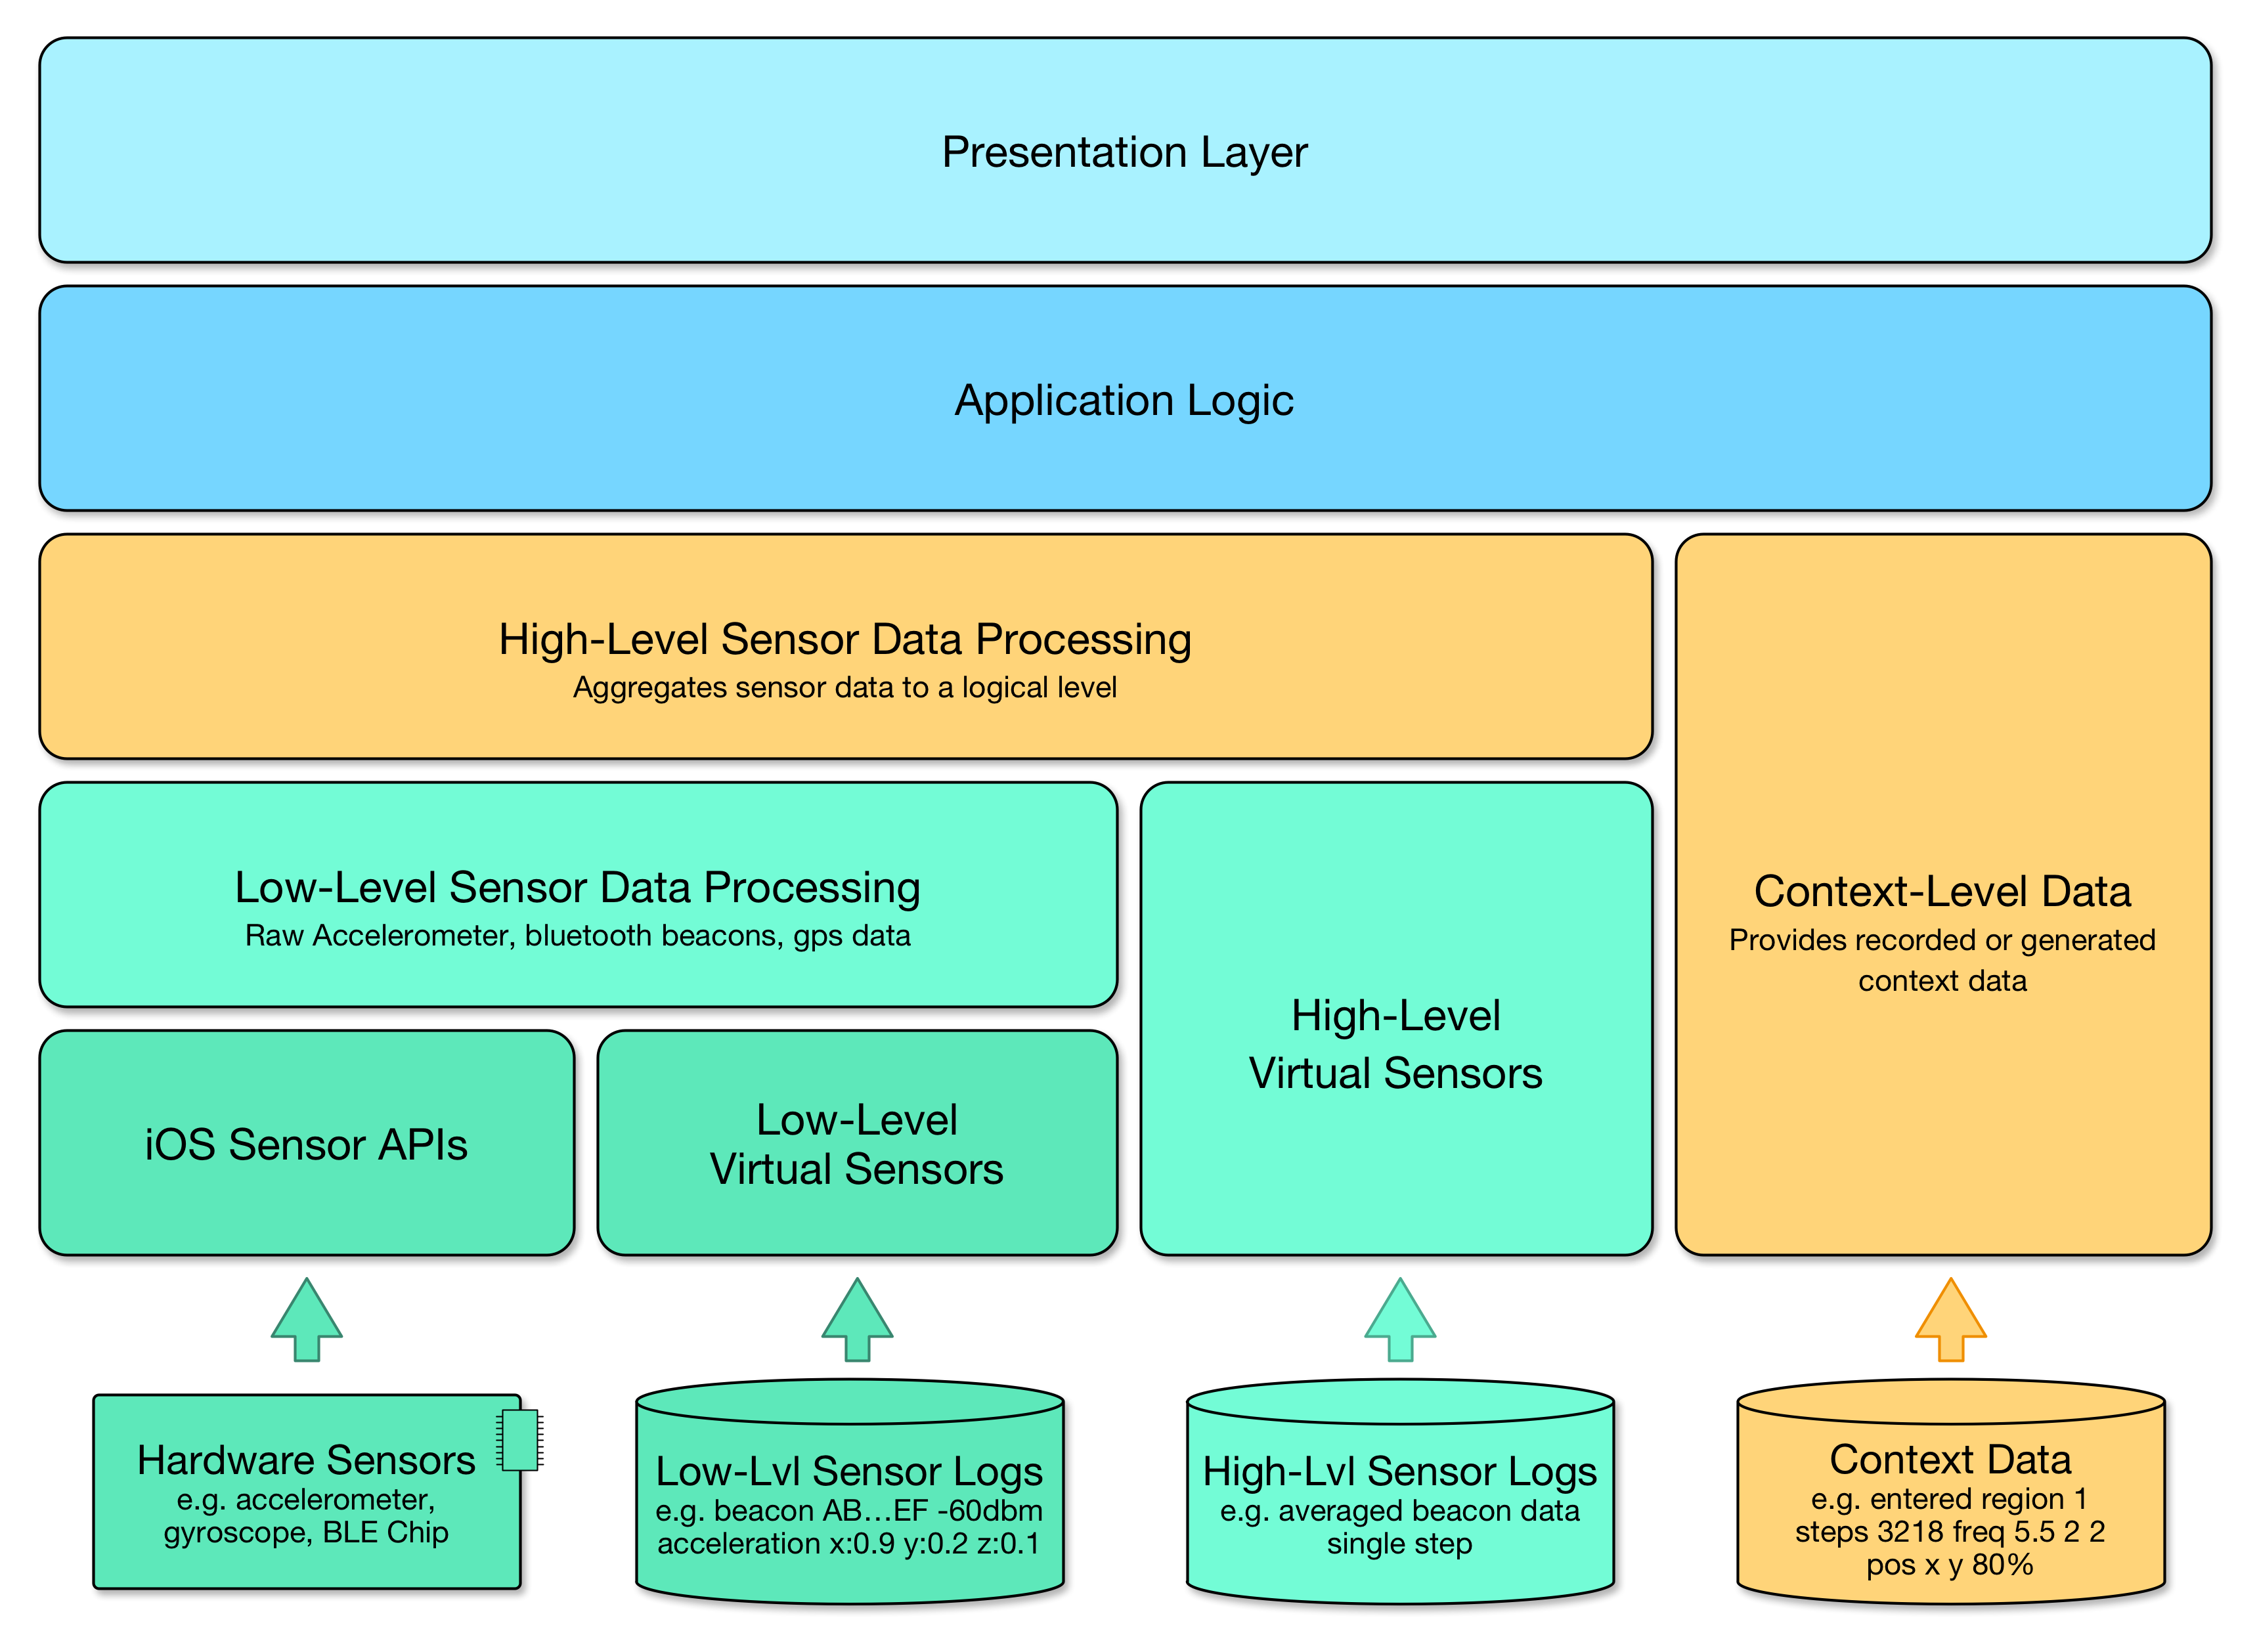
\includegraphics[width=0.9\textwidth]{layers-guide-refined-app.png}
\caption{Refined Layer Model}
\end{figure}

Virtual sensors of different levels for 
development 
automated testing
presentations  
easier migration to a different platform

\begin{figure}[H]
\centering
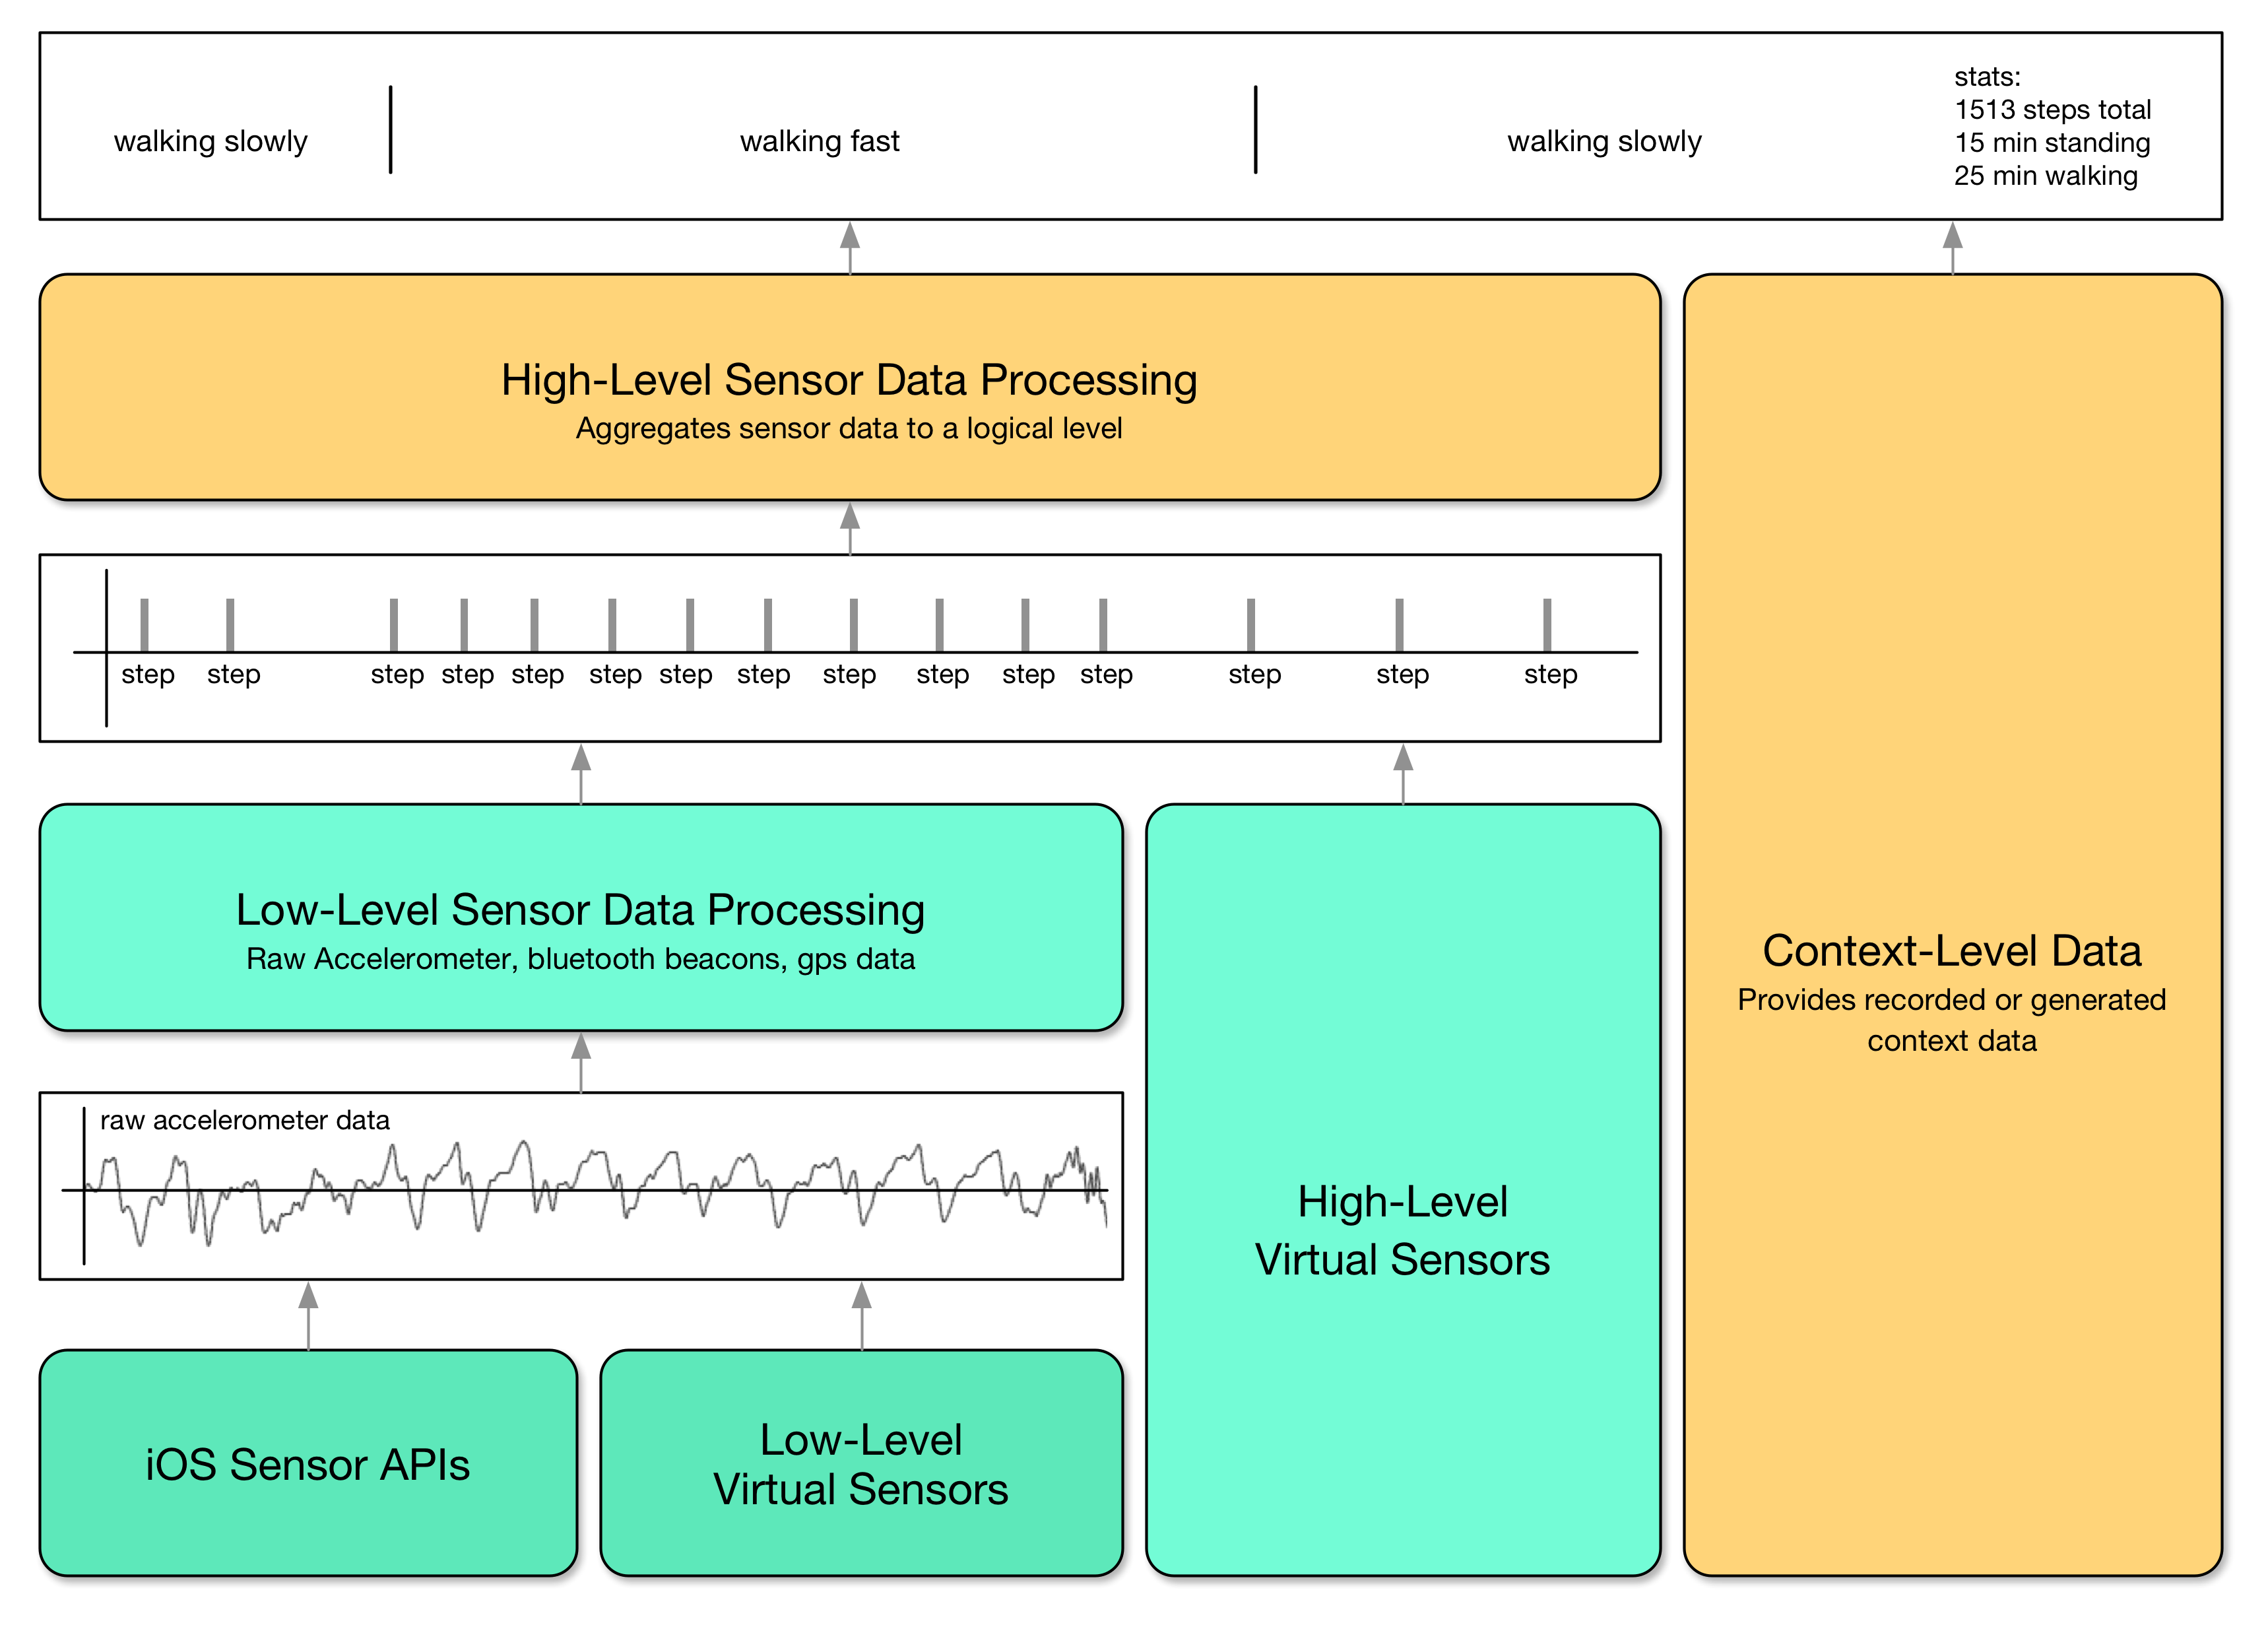
\includegraphics[width=0.9\textwidth]{layers-app-dataflow-accelerometer.png}
\caption{Data Flow between the lower Layers}
\end{figure}

Real Time Data

\begin{figure}[H]
\centering
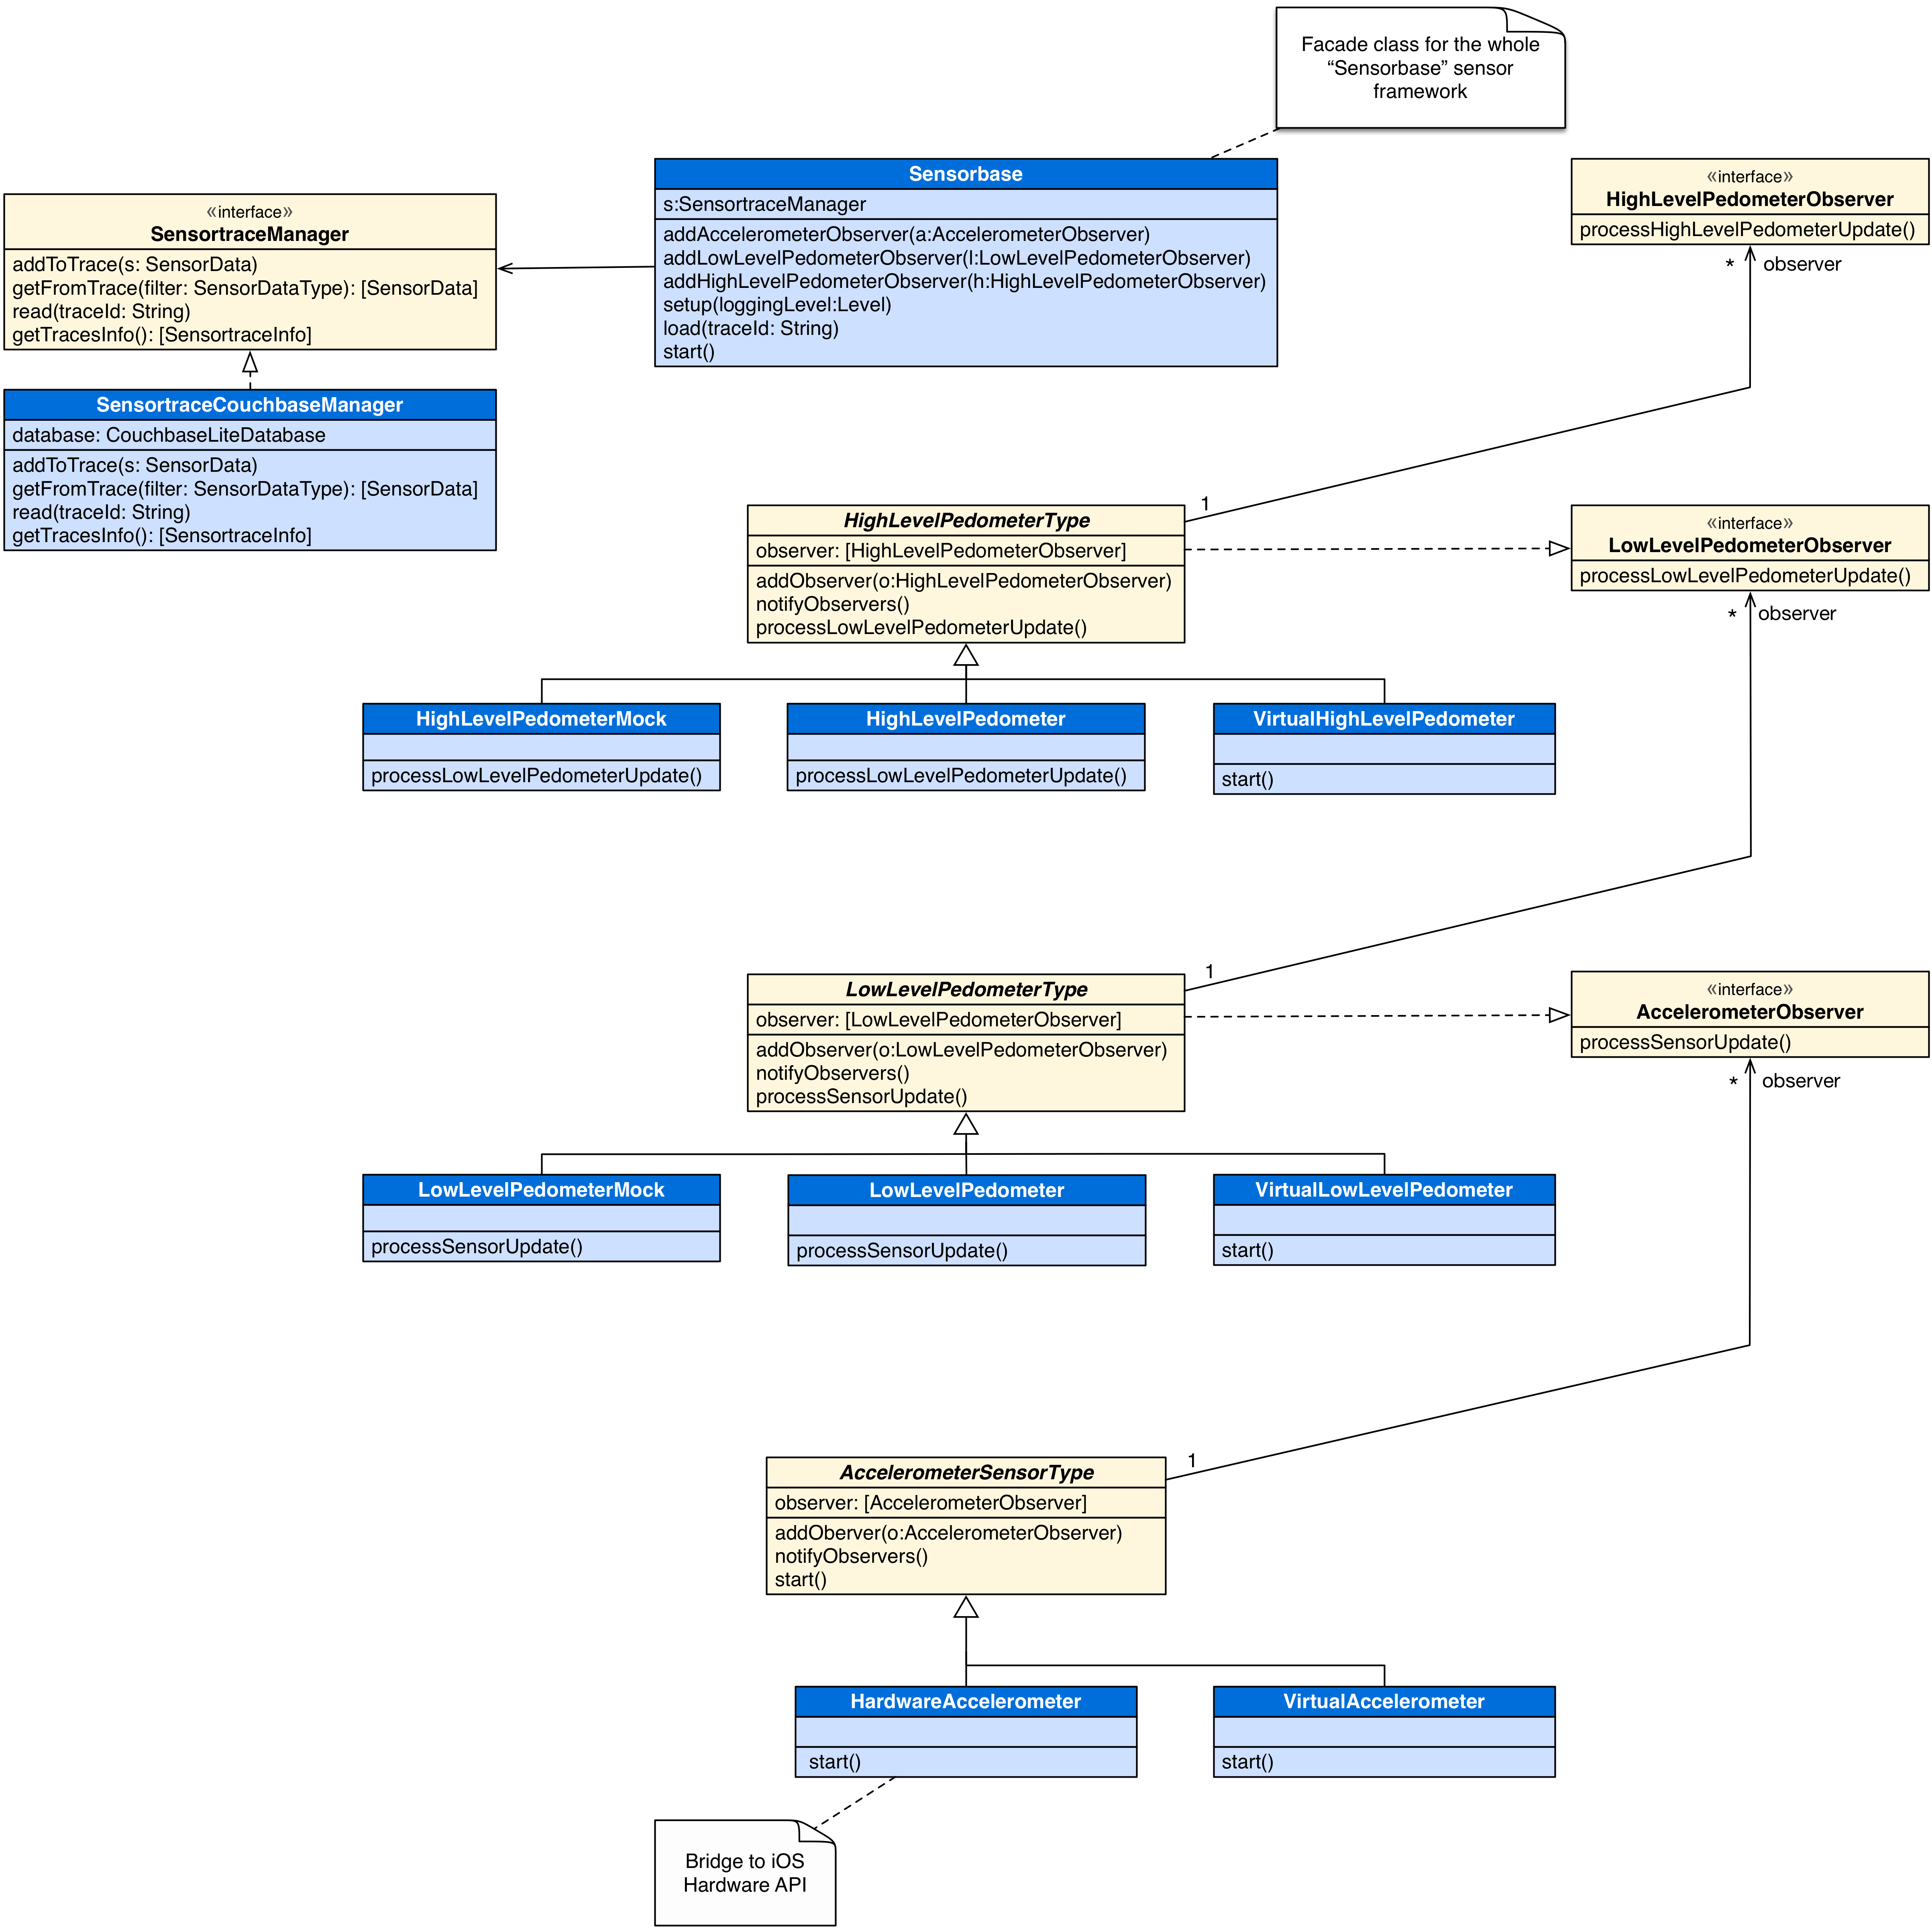
\includegraphics[width=1.0\textwidth]{class-diagram-guide-app.png}
\caption{Simplified Class Diagram for Sensor Data Processing}
\end{figure}

Mock: useful for Testing the underlying layer,
Adapter


\section{Sensors Layers}

Sensor data is saved to couchbase database.
Later access for replay (development), testing and presentations.
The backend can access this saved data for later analysis.

\section{Application Logic}

If not walking fast load and play current content.

If display is on show actions that user has to opt in, if display is off play automatically. 

\section{Presentation Layer}

Mockups
XCode Storyboard
Final App Screenshots